
%%%%%%%%%%%%%%%%%%%%%%%%%%%%%%%%%%%%%%%%%%%%%%%%%%%%%%%%%%%%%%%%%%%%%
%% This is a (brief) model paper using the achemso class
%% The document class accepts keyval options, which should include
%% the target journal and optionally the manuscript type. 
%%%%%%%%%%%%%%%%%%%%%%%%%%%%%%%%%%%%%%%%%%%%%%%%%%%%%%%%%%%%%%%%%%%%%
\documentclass[journal=jacsat,manuscript=article]{achemso}

%%%%%%%%%%%%%%%%%%%%%%%%%%%%%%%%%%%%%%%%%%%%%%%%%%%%%%%%%%%%%%%%%%%%%
%% Place any additional packages needed here. Only include packages
%% which are essential, to avoid problems later. Do NOT use any
%% packages which require e-TeX (for example etoolbox): the e-TeX
%% extensions are not currently available on the ACS conversion
%% servers.
%%%%%%%%%%%%%%%%%%%%%%%%%%%%%%%%%%%%%%%%%%%%%%%%%%%%%%%%%%%%%%%%%%%%%
\usepackage[version=3]{mhchem} % Formula subscripts using \ce{}
\usepackage{siunitx}
\usepackage{tabularx}
\usepackage{float}
\usepackage{booktabs}
\usepackage{subcaption}
\usepackage{amsmath}
\usepackage{amssymb}
\usepackage{amsfonts}
\usepackage{bm}
\usepackage{xfrac}
\usepackage{graphicx}

\usepackage[backend=biber,style=chem-acs, eprint=false, articletitle=true, note=false]{biblatex}

\DeclareSourcemap{
  \maps[datatype=bibtex, overwrite]{
    \map{
      \step[fieldset=isbn, null]
      \step[fieldset=issn, null]
      \step[fieldset=language, null]
    \step[fieldset=address, null]
    \step[fieldset=series, null]
    \step[fieldset=note, null]
    % \step[fieldset=Publisher, null]
    % \step[fieldset=language, null]
    }
  }
}

\ExecuteBibliographyOptions[misc]{eprint=true}
\addbibresource{references.bib} 




\usepackage[section]{placeins}

\DeclareMathOperator*{\argmax}{arg\,max}
\DeclareMathOperator*{\argmin}{arg\,min}
\newcommand{\SIci}[4]{\SI{#1}{#4},\ \SI{95}{\percent}C.I.\ [\numrange[range-phrase=---]{#2}{#3} \si{#4}]}
\newcommand{\numci}[3]{\num{#1},\ \SI{95}{\percent}C.I.\ [\numrange[range-phrase=---]{#2}{#3}]}
% Fancy table stuff
\newcommand{\nextitem}{\par\hspace*{\labelsep}\textbullet\hspace*{\labelsep}}
\newcolumntype{Z}{>{\centering\let\newline\\\arraybackslash\hspace{0pt}}X}

% Shorthand for features
\newcommand{\distlabel}{$dist.\ $}
\newcommand{\logitdistlabel}{$\mathrm{logit}(dist.)\ $}
\newcommand{\dihedlabel}{$dihed.\ $}

%%%%%%%%%%%%%%%%%%%%%%%%%%%%%%%%%%%%%%%%%%%%%%%%%%%%%%%%%%%%%%%%%%%%%
% % supplementary materials
% \usepackage{xr}
% \newcommand*\sref[1]{%
%     S\ref{#1}}
    
% \makeatletter
% \newcommand*{\addFileDependency}[1]{% argument=file name and extension
%   \typeout{(#1)}
%   \@addtofilelist{#1}
%   \IfFileExists{#1}{}{\typeout{No file #1.}}
% }
% \makeatother

% \newcommand*{\myexternaldocument}[1]{%
%     \externaldocument{#1}%
%     \addFileDependency{#1.tex}%
%     \addFileDependency{#1.aux}%
%     }


% \myexternaldocument{SI}
%%%%%%%%%%%%%%%%%%%%%%%%%%%%%%%%%%%%%%%%%%%%%%%%%%%%%%%%%%%%%%%%%%%%%

% \usepackage{caption}
% \captionsetup[table]{position=bottom} 
% \usepackage{subcaption}
% \usepackage{bm} % e.g., \bm(\mu)
% \usepackage{xfrac}  % e.g., \sfrac{1}{2}                   
% \usepackage{relsize} % e.g., \mathlarger 
% \usepackage{algorithm2e}
% \DeclareMathOperator*{\argmax}{arg\,max}
% \DeclareMathOperator*{\argmin}{arg\,min}

%%%%%%%%%%%%%%%%%%%%%%%%%%%%%%%%%%%%%%%%%%%%%%%%%%%%%%%%%%%%%%%%%%%%%
%% If issues arise when submitting your manuscript, you may want to
%% un-comment the next line. This provides information on the
%% version of every file you have used.
%%%%%%%%%%%%%%%%%%%%%%%%%%%%%%%%%%%%%%%%%%%%%%%%%%%%%%%%%%%%%%%%%%%%%
%%\listfiles

%%%%%%%%%%%%%%%%%%%%%%%%%%%%%%%%%%%%%%%%%%%%%%%%%%%%%%%%%%%%%%%%%%%%%
%% Place any additional macros here. Please use \newcommand* where
%% possible, and avoid layout-changing macros (which are not used
%% when typesetting).
%%%%%%%%%%%%%%%%%%%%%%%%%%%%%%%%%%%%%%%%%%%%%%%%%%%%%%%%%%%%%%%%%%%%%
\newcommand*\mycommand[1]{\texttt{\emph{#1}}}

%%%%%%%%%%%%%%%%%%%%%%%%%%%%%%%%%%%%%%%%%%%%%%%%%%%%%%%%%%%%%%%%%%%%%
%% Meta-data block
%% ---------------
%% Each author should be given as a separate \author command.
%%
%% Corresponding authors should have an e-mail given after the author
%% name as an \email command. Phone and fax numbers can be given
%% using \phone and \fax, respectively; this information is optional.
%%
%% The affiliation of authors is given after the authors; each
%% \affiliation command applies to all preceding authors not already
%% assigned an affiliation.
%%
%% The affiliation takes an option argument for the short name. This
%% will typically be something like "University of Somewhere".
%%
%% The \altaffiliation macro should be used for new address, etc.
%% On the other hand, \alsoaffiliation is used on a per author basis
%% when authors are associated with multiple institutions.
%%%%%%%%%%%%%%%%%%%%%%%%%%%%%%%%%%%%%%%%%%%%%%%%%%%%%%%%%%%%%%%%%%%%%

\author{Robert E. Arbon}
\altaffiliation{Redesign Science, 180 Varick St, New York, NY 10014, USA}
\affiliation[ed]{EaStCHEM School of Chemistry, David Brewster Road, Joseph Black Building, The King’s Buildings, Edinburgh, EH93FJ, UK}
\author{Yanchen Zhu}
\affiliation[ed]{EaStCHEM School of Chemistry, David Brewster Road, Joseph Black Building, The King’s Buildings, Edinburgh, EH93FJ, UK}
\author{Antonia S.J.S. Mey}
\email{antonia.mey@ed.ac.uk}
\affiliation[ed]{EaStCHEM School of Chemistry, David Brewster Road, Joseph Black Building, The King’s Buildings, Edinburgh, EH93FJ, UK}

%%%%%%%%%%%%%%%%%%%%%%%%%%%%%%%%%%%%%%%%%%%%%%%%%%%%%%%%%%%%%%%%%%%%%
%% The document title should be given as usual. Some journals require
%% a running title from the author: this should be supplied as an
%% optional argument to \title.
%%%%%%%%%%%%%%%%%%%%%%%%%%%%%%%%%%%%%%%%%%%%%%%%%%%%%%%%%%%%%%%%%%%%%
\title[]{Markov state models: to optimize or not to optimize}

%%%%%%%%%%%%%%%%%%%%%%%%%%%%%%%%%%%%%%%%%%%%%%%%%%%%%%%%%%%%%%%%%%%%%
%% Some journals require a list of abbreviations or keywords to be
%% supplied. These should be set up here, and will be printed after
%% the title and author information, if needed.
%%%%%%%%%%%%%%%%%%%%%%%%%%%%%%%%%%%%%%%%%%%%%%%%%%%%%%%%%%%%%%%%%%%%%
\abbreviations{MD, MSM, ML}
\keywords{American Chemical Society, \LaTeX}

%%%%%%%%%%%%%%%%%%%%%%%%%%%%%%%%%%%%%%%%%%%%%%%%%%%%%%%%%%%%%%%%%%%%%
%% The manuscript does not need to include \maketitle, which is
%% executed automatically.
%%%%%%%%%%%%%%%%%%%%%%%%%%%%%%%%%%%%%%%%%%%%%%%%%%%%%%%%%%%%%%%%%%%%%
\begin{document}

%%%%%%%%%%%%%%%%%%%%%%%%%%%%%%%%%%%%%%%%%%%%%%%%%%%%%%%%%%%%%%%%%%%%%
%% The "tocentry" environment can be used to create an entry for the
%% graphical table of contents. It is given here as some journals
%% require that it is printed as part of the abstract page. It will
%% be automatically moved as appropriate.
%%%%%%%%%%%%%%%%%%%%%%%%%%%%%%%%%%%%%%%%%%%%%%%%%%%%%%%%%%%%%%%%%%%%%
\begin{tocentry}

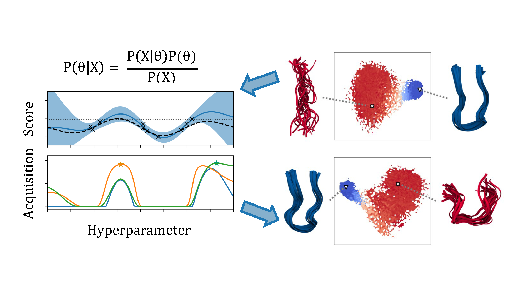
\includegraphics{figures/toc.eps}

\end{tocentry}

%%%%%%%%%%%%%%%%%%%%%%%%%%%%%%%%%%%%%%%%%%%%%%%%%%%%%%%%%%%%%%%%%%%%%
%% The abstract environment will automatically gobble the contents
%% if an abstract is not used by the target journal.
%%%%%%%%%%%%%%%%%%%%%%%%%%%%%%%%%%%%%%%%%%%%%%%%%%%%%%%%%%%%%%%%%%%%%
\begin{abstract}
Markov state models (MSM) are a popular statistical method for analyzing the conformational dynamics of proteins, including protein folding. With all statistical and machine learning (ML) models choices must be made about the modeling pipeline that cannot be directly learned from the data. These choices, or hyperparameters, are often evaluated by expert judgment or, in the case of MSMs, by maximizing variational scores such as the VAMP-2 score. Modern ML and statistical pipelines often use automatic hyperparameter selection techniques ranging from the simple: choosing the best score from a random selection of hyperparameters to the complex: optimization via e.g., Bayesian optimization. In this work, we ask whether it is possible to automatically select MSM models this way by estimating and analysing over \num{16000000} observations from over \num{280000} estimated MSMs. We find that differences in hyperparameters can change the physical interpretation of the optimization objective making automatic selection difficult. In addition, we find that enforcing conditions of equilibrium in the VAMP scores can result in inconsistent model selection. However, other parameters which specify the VAMP-2 score (lag time and number of relaxation processes scored) have only negligible influence on model selection.  We suggest that model observables and variational scores should only be a guide to model selection and that a full investigation of the MSM properties be undertaken when selecting hyperparameters. 
\end{abstract}

%%%%%%%%%%%%%%%%%%%%%%%%%%%%%%%%%%%%%%%%%%%%%%%%%%%%%%%%%%%%%%%%%%%%%
%% Start the main part of the manuscript here.
%%%%%%%%%%%%%%%%%%%%%%%%%%%%%%%%%%%%%%%%%%%%%%%%%%%%%%%%%%%%%%%%%%%%%
\section{Introduction}

Markov state models (MSMs) are a popular model for extracting kinetic information from unbiased molecular dynamics simulations. Recent studies include a wide range of applications, such as understanding protein association kinetics~\cite{cannariato_prediction_2022, chakrabarti_litmus_2022}, enzyme dynamics~\cite{koulgi_structural_2021}, ion binding mechanisms~\cite{dutta_distinct_2022, mckiernan_dynamical_2020}, hydrogen bond dynamics~\cite{ibrahim_dynamics_2022}, drug binding mechanisms for drug discovery~\cite{hu_discovery_2022, pantsar_decisive_2022, hempel_molecular_2021, tosstorff_study_2020, liu_silico_2021}, mutational effects on conformational dynamics~\cite{fernandez-quintero_mutation_2021, sharma_comparative_2020, juarez-jimenezDynamicDesignManipulation2020b, wapeesittipanAllostericEffectsCyclophilin2019a}, kinetics of intrinsically disordered proteins~\cite{paul_diversity_2020}, protein folding~\cite{zhou_molecular_2021}, and understanding allostery~\cite{tian_deciphering_2020, bowman_msmallosteric_2015, pontiggia_msmcprotein_2015}. Estimating an MSM proceeds~\cite{noe_markov_2019} by first collecting a data set of unbiased molecular dynamics (MD) simulations, then associating each molecular conformation with discrete states, counting transitions between states separated by the temporal resolution of the model (the lag time, $\tau$), and then deriving transition probabilities between states~\cite{trendelkamp-schroer_estimation_2015}. The final model is summarized by the transition matrix $\mathbf{T}$, where the elements $T_{ij}$ are the conditional probabilities of being in state $i$ at time $t$ and then transitioning to a state $j$ at time $t{+}\tau$: $T_{ij}(\tau){=}P(j, t{=}t{+}\tau| i, t{=}t)$.  The eigenvectors of the transition matrix represent the dynamic modes of the system as they relax to the equilibrium distribution. 

The entire process of transforming MD frames into a transition matrix involves making a number of modeling choices called \emph{hyperparameters}. Hyperparameters are differentiated from the \emph{parameters} of the model because the latter are calculated from the data via the optimization of a loss function (e.g., the negative log-likelihood), while the hyperparameters are chosen via expert judgment, or via some summary metric of the model\cite{feurer2019hyperparameter}. 
For MSMs, the important hyperparameters~\cite{Optimized_2016, scherer_variational_2019, husic_markov_2018} are which subset of atoms from the simulation to include (e.g., a protein loop, pocket, or other substructure of interest); the transformation of these coordinates into important features (e.g., residue-residue distances, backbone dihedral angles); dimensionality reduction onto a set of important collective variables (typically time-lagged independent component analysis, TICA~\cite{perez-hernandezIdentificationSlowMolecular2013a}, is used for this purpose. Other methods such as PCA~\cite{nagelSelectingFeaturesMarkov2023} and the generalization of TICA, Relaxation Mode Analysis~\cite{mitsutakeRelaxationModeAnalysis2018} have also been used, but we focus on the most commonly use method which is TICA.  Finally how to define discrete states from these collective variables (via some clustering algorithm such as K-Means). Therefore, the parameters of an MSM are the conditional probabilities in the transition matrix, $T_{ij}$, whereas the hyperparameters are all the choices (choice of features, clustering algorithm, etc.) that gave us the specific state definitions used in the likelihood maximization step.   

Hyperparameter optimization is an important part of modern statistical and machine learning (ML) analysis pipelines~\cite{feurer2019hyperparameter, bergstra_jamesbergstra_random_2012, bergstra_making_2013, bergstraAlgorithmsHyperParameterOptimizationa} as hyperparameters can have a strong impact of the performance of a model. There are several methods to find the optimal set of hyperparameters, from exhaustively searching a uniformly spaced grid of choices~\cite{c1997montgomery} or randomly selected from a predefined search space~\cite{bergstra_jamesbergstra_random_2012}, evolutionary and population algorithms~\cite{simon2013evolutionary, kennedyParticleSwarmOptimization1995, eberhart1998comparison, hansenCMAEvolutionStrategy2016} to active learning approaches such as Bayesian optimization~\cite{hutterSequentialModelbasedOptimization2011, bergstraAlgorithmsHyperParameterOptimizationa, NIPS2012_4522, bergstraMakingScienceModel2013}.

No `ground truth' data exist for MSMs used for the analysis of protein MD trajectories, so the accuracy of the eigenvectors cannot be judged absolutely. However, a family of variational scores exist which provide a means to compare the relative accuracy of MSMs and thus allow hyperparameter optimization to be performed. The first score to be developed was the cross-validated generalized matrix Rayleigh quotient~\cite{mcgibbonVariationalCrossvalidationSlow2015}, GRMQ, which pertains to reversible MSMs; while the variational approach to Markov processes (VAMP) scores~\cite{wuVariationalApproachLearning2020c,scherer_variational_2019} extended these ideas to both reversible, non-reversible and non-stationary models. These scores measure how well the eigenvectors of the transition matrix (singular vectors in the case of non-reversible models) approximate the `true' eigenvectors in a variational sense i.e., the higher the score, the better the approximation. Thus, optimization of eigenvectors can proceed without the need for a `ground truth' to compare to.   

To use a variational score, it is necessary to specify the lag time ($\tau$) of the MSM and the number of slow relaxation modes to optimize ($k$), and then estimate the MSM with different hyperparameters. The `best' set of hyperparameters is the one with the highest variational score. In the case of the VAMP-E score, one may also add $k$ to the list of hyperparameters to optimize. 

This procedure removes the need for potentially arbitrary hyperparameter selection with the concomitant risk of findings that are not robust to changes in modeling assumptions. This method has been used in a number of different studies~\cite{A_Minimum_2018, Adaptive_M2020, High-Resol2019, Maximizing2018, Modeling_t2017, Optimized_2016, Quantitati2018, VAMPnets_f2018, Variationa2018, Ward_Clust2017}. In addition, it has allowed investigations into the roles of various hyperparameters and for other methods for hyperparameter selection to be developed. In Husic et al.~
\cite{Ward_Clust2017} the authors used the GMRQ to show that the Ward and K-means methods are optimal for clustering conformations for MSMs. In Husic et al.~\cite{Optimized_2016} the authors performed a sensitivity analysis of the GMRQ  in order to determine the sensitivity of hyperparameters in describing protein folding.  An extension of the VAMP score by Scherer et al.~\cite{scherer_variational_2019} showed that the optimal set of features could be selected before going through the full MSM creation and scoring pipeline. However, using variational optimization is not the only method for principled construction of MSMs, see for example Nagel et al.~\cite{nagelSelectingFeaturesMarkov2023, nagelBenchmarkMarkovState2023}'s careful construction of an MSM of the Villin headpiece. In this work the authors stress the need of models to produce explanations with sufficient spatial and temporal resolution to resolve metastable states and folding mechanism. In addition they note the need to calibrate against different physical conditions such as temperature. 

It is tempting to think that with a single model metric and state-of-the-art ML optimization software, it should be possible to form an automatic pipeline wherein simulation data are fed in, and a single optimized MSM describing the kinetics and thermodynamics of the system comes out. However, many detailed questions need to be answered before such a pipeline is possible. First, do variational scores refer to the same relaxation mode across all possible combinations of hyperparameters?  It is possible that with certain combinations of hyperparameters, the eigenvectors could describe different relaxation modes. It is therefore possible that the variational scores do not compare the same set of processes across different sets of hyperparameters. Second, the MSM lag time and number of scored processes interest will affect the variational scores --- does this have any material effect on how we rank different sets of hyperparameters? Third, do we need variational scores to optimize models at all?  Will model observables, such as the implied timescales suffice to optimize MSMs?  Finally, does hyperparameter optimization work for MSMs compared to randomly sampling hyperparameters?  Here, we use a common method (Bayesian optimization with tree Parzen estimators) for optimizing machine learning models to find optimal hyperparameters. 


The remainder of this work is structured as follows.  In the next section, we cover the necessary theory to understand MSMs and Bayesian optimization of hyperparameters; this is followed by the methods; and results analysis. The paper is concluded with some recommendations based on our findings. 

\section{Theory}\label{theory}
\subsection{Markov state models}
\subsubsection{Overview}

What follows is a brief overview of the theory of Markov state models (MSMs), for a more detailed picture see some of the many good references~\cite{prinzMarkovModelsMolecular2011, trendelkamp-schroer_estimation_2015,husic_markov_2018}. MSMs describe the first-order conformational kinetics of a system by specifying the conditional probability of transitioning from a state $i$ at a time $t$ to a state $j$ at a time $t+\tau$  later. This information is summarized in the transition matrix $T_{ij}(\tau) = P(j, t+\tau | i, t)$. Each state, $i$, is a collection of conformations which have similar kinetic properties. The transition matrix is a finite and discrete representation of the underlying Markovian transfer operator, $\mathcal{T}(\tau)$, which describes the dynamics of the system. The first left eigenvector $\phi_1$ (in descending eigenvalue order $\lambda_i$, with $\lambda_{1} = 1$) corresponds to the stationary or equilibrium distribution, which we also label $\pi$; the second left eigenvector, $\phi_2$ corresponds to the slowest conformational relaxation process; the third is the next slowest relaxation process and so on. The corresponding right eigenvectors, $\psi_{i}$ are normalized by $\pi$ (so $\psi_{1} = 1$ for all states). The eigenvalues are related to the timescales of these relaxation processes by: $t_{i} = -\tau/\log{\lambda_i}$.  The transition matrix is said to be reversible if it obeys detailed balance $\pi_i T_{ij}=\pi_j T_{ji}$. 

The transition matrix is specified with respect to a set of $p$ basis states, $\chi_1, \chi_2, ..., \chi_p$ which we denote as a vector $\bm{\chi}$. In what follows, the basis states are assumed to be discrete and orthonormal and each one corresponds to a small region of conformational space.  Each frame of an MD trajectory can be mapped to one of these basis states and these discretized MD trajectories form the data from which the transition matrix is estimated.

The mapping between the atomic coordinates $\mathbf{x}$ and the basis states we call $f(\mathbf{x}; \bm{\theta}) =  \bm{\chi}$ where $\bm{\theta}$ is a vector of parameters of that mapping. For example, $f$ may involve projecting coordinates onto the backbone dihedral angles of a protein, followed by clustering into \num{100} discrete states using k-means clustering. The MSM is then specified with a lag time of \SI{10}{\nano\second}. The parameters of the MSM are the $100 \times 100 = 10000$ elements of $\mathbf{T}$, while the hyperparameters are $\bm{\theta}=($backbone dihedrals, K-Means, $100)$ where the elements correspond to the feature, clustering method, number of basis states respectively.  

\subsubsection{Estimating a reversible MSM}

The first step in estimating a reversible MSM is projecting the MD trajectories onto the proposed basis states, $\bm{\chi}$. Transitions between each basis state at time $t$ and time $t + \tau$ are tabulated in a count matrix, $\mathbf{C}_{0t}$ (the subscript $0$ and $t$ refer to the fact that the counted transitions are between $t$ and $t+\tau$).
The population of each state is given by the diagonal matrix, $\mathbf{C}_{00}$ calculated as the row-sum of the count matrix $[\mathbf{C}_{00}]_{i, i} = \sum_j [\mathbf{C}_{0t}]_{i, j}$.  A \emph{non-reversible} transition matrix is then given by $\mathbf{T}^{\mathrm{irrev}} = \mathbf{C}_{0t}\mathbf{C}_{00}^{-1}$. It is non-reversible because of the finite amount of simulation data will not be in perfect equilibrium. A transition matrix and stationary vector which obey detailed balance, $\mathbf{T}^{\mathrm{rev}}$ and $\bm{\pi}^{\mathrm{rev}}$, can be estimated from $\mathbf{C}_{0t}$ using maximum likelihood estimation with constraints~\cite{trendelkamp-schroer_estimation_2015}. The constraints ensure that detailed balance is obeyed by $\mathbf{T}$ and its dynamics are reversible.  However, once $\mathbf{T}^{\mathrm{rev}}$ and $\bm{\pi}^{\mathrm{rev}}$ have been estimated, they are now inconsistent with $\mathbf{C}_{0t}$ and $\mathbf{C}_{00}$, as obtained from the MD trajectory.

\subsubsection{Variational scores}

The key idea behind variational scores is that approximations to the true eigenvectors of the transition matrix will give rise to eigenvalues which are bounded from above by the true eigenvalues, specifically~\cite{mcgibbonVariationalCrossvalidationSlow2015, wuVariationalApproachLearning2020c}: 
\begin{equation}\label{eqn:var_principle}
    \sum_{i=1}^{k}\hat{\lambda}_{i}^{r} \leq \sum_{i=1}^{k}\lambda_{i}^{r},
\end{equation}
where $\hat{\lambda}$ are the eigenvalues estimated from an approximate basis set $\bm{\chi}$ and $\lambda$ are the true eigenvalues. The sum runs over the first $k$ eigenvalues, which are typically the dominant slow relaxation processes that one is interested in approximating; while $r$ is some arbitrary positive integer~\cite{wuVariationalApproachLearning2020c}.

When $r=1$ and the model is assumed to be stationary~\cite{mcgibbonVariationalCrossvalidationSlow2015}, the left-hand side of Equation~\ref{eqn:var_principle} is known as the Generalized Matrix Rayleigh Quotient (GMRQ):

\begin{equation}
    \operatorname{GMRQ}(\bm{\theta}) = \operatorname{Tr}\left[(\mathbf{U}^{T}\mathbf{C}_{01}\mathbf{U})(\mathbf{U}^{T}\mathbf{C}_{00}^\mathbf{U})^{-1}\right], \label{eqn:gmrq_def}
\end{equation}

where $\mathbf{U}$ is the matrix of eigenvectors of $\mathbf{T}$. The functional dependence of the GMRQ on $\bm{\theta}$ is to emphasize that the eigenvectors and count matrices are dependent on the hyperparameters. 

The variational approach to Markov processes placed reversible and stationary MSMs in a broader context of Koopman models which may or may not be reversible or stationary.  In this context there is a family of variational scores, differentiated by a positive integer $r$: 
\begin{equation}
     \operatorname{VAMP-r}(k, \bm{\theta}) = \left \| (\mathbf{U}^{T}\mathbf{C}_{00}\mathbf{U})^{-\frac{1}{2}}(\mathbf{U}^{T}\mathbf{C}_{0t}\mathbf{V})(\mathbf{V}^{T}\mathbf{C}_{tt}\mathbf{V})^{-\frac{1}{2}} \right \|_{r}^{r}, \label{eqn:vamp_def}
\end{equation}

where $\mathbf{C}_{tt}$ is the column-sum of the count matrix $[\mathbf{C}_{tt}]_{i, i} = \sum_i [\mathbf{C}_{0t}]_{i, j}$; $\mathbf{U}$ and $\mathbf{V}$ are the left and right singular vectors of the transition matrix. The functional dependence on $\bm{\theta}$ comes from its influence on the basis states which in turn determines the singular vectors; $k$ is the number of singular vectors being scored and determines the dimensions of $\mathbf{U}$ and $\mathbf{V}$.  

The matrix norm denotes takes the $r$\textsuperscript{th} power of the Schatten-r norm: 
where,
\begin{equation}
    \left | \boldsymbol{T} \right |_{r}^{r} = \sum_{i}s_i^r(\boldsymbol{T})
\end{equation}
and $s_i$ are the singular values of a matrix, $\boldsymbol{T}$. 

If the data are stationary, reversible and $r{=}1$ this is equivalent to the GMRQ. With $r{=}2$ this expression measures the kinetic variance~\cite{noeKineticDistanceKinetic2015} captured by the basis sets. The VAMP scores have also been adapted to score the models based on the type of feature alone (rather than scoring the full MSM)~\cite{scherer_variational_2019}. 

As timescales are monotonic functions of the eigenvalues, maximizing the sum of the timescales also maximizes the VAMP scores. 


\subsubsection{Cross-validation and bootstrapping}

Hyperparameters should be chosen to maximize the performance of a model on unseen data. Simply maximizing the variational score on the data used to fit the model (training data) may result in eigenvectors which describe this data well but do not generalize to new data generated by the same system. This is known as over-fitting and is a well-documented phenomenon~\cite{friedman2001elements}. To overcome this problem the estimated VAMP scores should be close to those attained on unseen data. One estimation method is to withhold a portion of the data (test set) and calculate the variational scores on this set. While accurate, it requires ignoring a large proportion of the data for training purposes, which may be wasteful when there are only a handful of observed transitions which we are interested in modeling. 

Two other popular methods, which make more efficient use of the available data,  are cross-validation~\cite{arlotSurveyCrossvalidationProcedures2009} and bootstrapping~\cite{efronIntroductionBootstrap1993}. The estimators for the variational scores (Equations~\ref{eqn:gmrq_def} and \ref{eqn:vamp_def}) were both adapted to be used with cross-validation\cite{wuVariationalApproachLearning2020c, mcgibbonVariationalCrossvalidationSlow2015}: data is randomly split into two equally sized subsets. The eigenvectors $\mathbf{U}/\mathbf{V}$ are calculated on one set, while the count matrices $\mathbf{C}_{00/0t/tt}$ are calculated on the other set.  This is repeated $N_c$ times (e.g.,~\cite{scherer_variational_2019} $N_c =50$) and an average of the VAMP scores is taken.

The bootstrap does not require a reformulation of estimators. Instead, a number, $N_b$, of new data sets are created from the original data set (e.g.,~\cite{efronIntroductionBootstrap1993} $N_b = 100 - 1000$) and the mean or median of variational scores on each of these data sets used. To create the bootstrapped data sets, 
trajectories are split into small independent subtrajectories. The subtrajectories are sampled \emph{with replacement} to create a new bootstrapped data set of the same size as the original. 

% Both techniques are used in practice; however, the approach we advocate is the bootstrap, primarily because the data splitting used in cross-validation means only \SI{50}{\percent} of the data is used in estimation.  This decreases the precision of the estimated eigenvectors, and, for particularly rare events increases the likelihood that conformational transitions may only occur in a portion of the data at a time. The sub-spaces spanned by the $\mathbf{U}/\mathbf{V}$ and $\mathbf{C}_{00/0t/tt}$ may be different, invalidating the score. In addition, the bootstrap can be used for a wider variety of observables.
 
\subsection{Hyperparameter optimization}

\subsubsection{Methods for optimizing hyperparameters}

Finding the best set of hyperparameters $\bm{\theta}$ using either the VAMP scores or implied timescales (we will use the term \emph{response} generally), is a black-box optimization problem.  It is black box because we do not have access to the gradients, $\nabla_{\bm{\theta}} \operatorname{VAMP-r}(k, \bm{\theta})$, which would facilitate a gradient-based optimization. There are three broad classes of optimization techniques in this case: exhaustive searching, model-based searching and population-based algorithms. 

Examples of exhaustive searching are grid search where hyperparameters are taken from a uniformly placed grid over the hyperparameter search space, and random search, where hyperparameters are randomly sampled from the search space. 

Grid search is an effective strategy when the response is sensitive to all the hyperparameters.  However, it has poor scaling with the number of hyperparameters ($N^d$, where $N$ is the number of grid points per hyperparameter and $d$ is the number of hyperparameters), so when only a small subset of hyperparameters are relevant, random search is more efficient~\cite{bergstra_jamesbergstra_random_2012}.  

Model-based search algorithms construct surrogate models of the mapping between the hyperparameters and the model response which are cheap to evaluate and optimize, and use these models to guide hyperparameters to test. Examples include Bayesian optimization with either a Gaussian process or a  tree Parzen estimator (TPE) as the surrogate model~\cite{bergstraAlgorithmsHyperParameterOptimizationa}.  The third class of optimization algorithms is population algorithms, which include evolutionary algorithms~\cite{simon2013evolutionary,eberhart1998comparison}, particle swarm optimization~\cite{kennedyParticleSwarmOptimization1995,eberhart1998comparison} and covariance matrix adaption~\cite{hansenCMAEvolutionStrategy2016}, these will not be explored here further. 

\subsubsection{Bayesian optimization with tree-structured Parzen estimators}
We chose tree-structured Parzen estimators to perform optimization because they easily handle numerical as well as categorical hyperparameters and can easily model conditional hyperparameter search spaces (i.e., choosing hyperparameters based on the choices of other hyperparameters) - this latter feature is the `tree-structure' referred to in the name of the method. 

Bayesian Optimization with TPE optimization proceeds as follows. 
\begin{enumerate}
    \item Randomly sample a small set of hyperparameters and measure the response of the resulting MSMs. This gives a hyperparameter trial data set $\mathcal{D}_{n}=\left\{(y_1, \bm{\theta}_1),  \ldots (y_n, \bm{\theta}_n) \right \}$ where $y$ is the model response.
    \item Construct a model of the probability of the hyperparameters, given the response, $p(\bm{\theta}|y)$ as two separate probability density functions: 
    \begin{equation}
        p(\bm{\theta} \mid y)= \begin{cases}\ell(\bm{\theta}) & \text { if } y>y^* \\ g(\bm{\theta}) & \text { if } y \leq y^*\end{cases}, 
    \end{equation}
    where $y^{*}$ is some user specified quantile, $\gamma$ of the observations.  $l$ and $g$ are probability models of the `good' and `bad' hyperparameters respectively and are explained more fully below. \label{itm:model_theta} 
    \item To find the $n+1$\textsuperscript{th} value of $\bm{\theta}$ we maximize the \emph{Expected Improvement}: $\mathrm{EI}_{y^{*}}(\bm{\theta}) = \mathbb{E}_{\bm{\theta}}\left[\max{(y(\bm{\theta})-y^{*}, 0)} \right ]\propto\left(\gamma+\frac{\ell(x)}{g(x)}(1-\gamma)\right)^{-1}$.
    \item Evaluate $\bm{\theta}_{n+1}$ on the MSM and measure the response, $y_{n+1}$, add $\left( \bm{\theta}_{n+1}, y_{n+1}\right)$ to the hyperparameter trial data set. \label{itm:augment_data}
    \item Repeat steps \ref{itm:model_theta} to \ref{itm:augment_data} until convergence in the maximum value of $y$ is reached.   
    
\end{enumerate}

The functions $l$ and $g$ are Parzen estimators, otherwise known as kernel density estimators. These model the probability density of $\bm{\theta}$ by placing truncated Gaussian distributions over each observation of a continuous hyperparameter, and a categorical distribution proportional to the observed counts of each level for each discrete hyperparameter. More details can be found in Bergstra et al.~\cite{bergstraAlgorithmsHyperParameterOptimizationa, bergstraMakingScienceModel2013}. 

This method can also be extended to dual objective functions, i.e., when optimizing two (or more) responses, $\mathbf{y}_i=(y^1_i, y^2_i)$, for the same model. In this case the `best' solutions form a Pareto set. Any member of a Pareto set, $\mathbf{y}_k$, has both responses superior to all other trials ($y^1_k>y^1_i, y^2_k>y^2_i$ for all $i$) but which are only superior to other members of the set in one response ($y^1_k>y^1_{k^{\prime}}$ or $y^2_k>y^2_{k^{\prime}}$ for $k$ and $k^{\prime}$ in the Pareto set). For dual-objective optimization the acquisition function was the expected hyper-volume improvement~\cite{ozaki_multitpe_2022}. This function tries to find hyperparameters which expand the Pareto set. The splitting of observations into two sets is complex, see Ozaki et al.~\cite{ozaki_multitpe_2022} for details on the splitting algorithm.



\section{Methods}
To answer our research questions we estimated a large number of Markov state models with different hyperparameters, measured their observables and analysed the results. The workflow may be summarized as follows.  We used existing molecular dynamics trajectories of Chignolin and BBA and fit MSMs with 140 randomly sampled hyperparameters (\emph{hyperparameter trials}) and recorded implied timescales, eigenvalues, and VAMP-2 scores for a range of different lag times ($\tau$). Each observable was estimated with confidence intervals using bootstrapping. This data constituted our \emph{hyperparameter trial data set} and was analyzed in the first, second and last results subsections. A `toy' three-state MSM model was constructed to highlight with the VAMP-2 score, for reversible transition matrix estimation. We then performed Bayesian optimization with a TPE surrogate function, with a variety of different objective functions, and using the hyperparameter trial data set to initialize the surrogate function. These results are discussed in the third part of the results.


\subsection{Molecular dynamics}

We use simulation data of the fast-folding proteins Chignolin (CLN025) and BBA, two of the twelve fast-folding proteins which have become the \textit{de facto} benchmark data set for testing molecular kinetics methods. The methods used to create this data are described elsewhere~\cite{lindorff-larsen_how_2011}. Important information on the data is shown in Table~\ref{tab:data_description}: the average folding time was calculated by the authors~\cite{lindorff-larsen_how_2011}; the sub-trajectory length and number of sub-trajectories correspond to the data splitting used in the bootstrapping procedure. 

\begin{table}
    \caption{\textbf{Description of molecular dynamics data}}
    \begin{tabularx}{\textwidth}{llXXXXX}
    \toprule
    Name & PDB & Simulation time (\si{\micro\second}) & Average folding time (\si{\micro\second}) & No. Residues & Sub-trajectory length (\si{\micro\second}) & No. sub-trajectories \\
    \midrule
    BBA                 & 1FME      & \num{325}     & \num{18}  & 28 & \num{2} & 164 \\
    Chignolin           & 5AWL    & \num{106}     & \num{0.6}  & 10 & 2 & 53 \\ 
    \bottomrule
    \end{tabularx}
    \label{tab:data_description}
\end{table}

\subsection{Markov state models}
MSMs were estimated using PyEMMA version 2.5.7~\cite{schererPyEMMASoftwarePackage2015a} and used a standard pipeline when focusing on the slow relaxation processes~\cite{noe_markov_2019, husic_markov_2018}: 
\begin{enumerate}
    \item Project molecular dynamics (MD) trajectories onto a set of features. 
    \item Reduce the dimension of the feature trajectories using TICA with a lag time $\tau_{\mathrm{TICA}}$ by projecting onto the first $m$ TICA coordinates. 
    \item The frames of the TICA trajectories were clustered using the k-means algorithm into $n$ discrete microstates. 
    \item A reversible, maximum likelihood MSM was then estimated. 
\end{enumerate}
To save on memory and compute resources the data was subset in parts of the MSM estimation. The MD trajectories were first strided so that the time between each frame was \SI{1}{\nano\second} in line with previous analysis in the literature~\cite{sultan_mdstride_2018,beauchamp_mdstride_2013}. The cluster centers were estimated on frames separated by \SI{10} {\nano\second}, i.e. only the 0\textsuperscript{th}, 10\textsuperscript{th}, etc. frames were used for estimating the cluster centers. 

The uncertainty for model observables was estimated using bootstrap with \num{100} bootstrap samples. The point estimate and error bars were calculated as the median,   \SI{2.5}{\percent} and \SI{97.5}{\percent} quantiles of the distribution from the bootstrap samples.

\subsection{Hyperparameters and scoring}
\num{140} different hyperparameters were randomly sampled from the search space described by Table~\ref{tab:search_space}. Each set of hyperparameters and their corresponding model observables are known as a \emph{hyperparameter trial}. Three different features, $f$, were used: 
\begin{enumerate}
    \item dihedrals feature (`dihed.'): the sine and cosine of the $\phi$, $\psi$ and $\chi_{1-5}$ angles of the amino acid residues;
    \item contact distance feature (`dist.'): the distance between all pairs of residues separated by three or more residues; \label{itm:cont_dist_feat}
    \item logistic distance feature (`logit(dist.)'): the same as feature~\ref{itm:cont_dist_feat} but with a logistic transform applied to the distance ($d$): $\mathrm{logit}(d) = [1+\exp{(s(d-c))}]^{-1}$, where center, $c$, and steepness $s$,  have units of \si{\angstrom} and \si{\per\angstrom} respectively.
\end{enumerate}
The logistic distance feature may be described as a `soft' or `fuzzy' contact map: it takes on the value $0$ for $d \gg c$ and a value of $1$ for $d\ll c$, and varies between these two extremes in the neighborhood of $c$ with a steepness determined by $s$. The definitions of the contact distances ($d$) were either the closest heavy-atom distance ($X$-$X$) or the distance between the $\alpha$-Carbons (C$\alpha$-C$\alpha$). The TICA eigenvectors were scaled by their eigenvalues ($\lambda$) so that distances in TICA space correspond to kinetic distances~\cite{noeKineticDistanceKinetic2015}.

The number of trials was approximately proportional to the number of hyperparameters for each feature: 20 trials for the dihedral feature, 40 for the contact distances (20 for each value of the contact distance scheme: $X$-$X$,  C$\alpha$-C$\alpha$), and 80 for the logistic transformation of contact distances (which, in addition to the two distance scheme values, has two other hyperparameters, $c$ and $s$). 

For each trial,  $\bm{\theta} = (f, \tau_{\mathrm{T}}, m, n, c, s)$,  an MSM was estimated using the procedure above with a range of Markov lag-times, $\tau$: \SI{1}{\nano\second}, \SI{11}{\nano\second}, ..., \SI{101}{\nano\second}. For each combination of $\bm{\theta}$ and  $\tau$ the slowest \numrange{2}{21} eigenvectors were scored using the VAMP-2$(k, \bm{\theta})$ (Equation~\ref{eqn:vamp_def}) and  VAMP-2$_{eq}(k, \bm{\theta})$ score (Equation~\ref{eqn:vamp_eq_def}):
\begin{equation}
    \operatorname{VAMP-2_{eq}}(k, \bm{\theta}) = \sum_{i=1}^{k}\lambda_{i}^{2}, \label{eqn:vamp_eq_def}
\end{equation}
where $\lambda$ are the eigenvalues of the MSM transition matrix which obey detailed balance, along with the implied timescales, $t_i$.  Each of these observations was estimated as the median of $N_b=100$ bootstrapped samples. 

VAMP-2$(k, \bm{\theta})$ and VAMP-2$_{eq}(k, \bm{\theta})$ will be abbreviated as VAMP2$(k)$ and VAMP2$_{eq}(k)$ from here on, the dependence on $\bm{\theta}$ being assumed. 

Selected models were validated by: 
\begin{enumerate}
    \item inspection of structures sampled from microstates which had the most extreme values of $\psi_2$;
    \item inspection of both $\psi_2$ and a two-state coarse grained model in the space of the first two TICA components;
    \item a plot of the mean first passage time as a function of the lag time (as suggested in Suarez et al.~\cite{suarezWhatMarkovState2021});
    \item implied timescales as a function of the lag time, $\tau$.
\end{enumerate} 

The validation details of the selected models can be found in the supplementary information. 

\begin{table}
    \centering
    \begin{tabularx}{\textwidth}{lXXXX}
    \toprule
    \textbf{Features}, ($f$)  & & & &\\
    Dihedral angles & \textsc{Which} & & &\\
    & \multicolumn{4}{l}{$dihed.=\phi, \psi, \chi_{1}, \ldots, \chi_{5}$ (sine and cosine transformation)} \\
    Contact distances &  \textsc{Definition}, ($d$) & \textsc{Transform}& \textsc{Center} ($c$, \si{\angstrom}) & \textsc{Steepness} ($s$, \si{\per\angstrom}) \\

     & \nextitem $X$-$X$  \nextitem C$\alpha$-C$\alpha$ & \nextitem $\mathrm{logit}(dist.)$ \nextitem $dist.$ &  \numrange{3}{15} & \numrange{0.01}{5} \\
    \midrule
    \textbf{Decomposition} & \textsc{Eigenvectors}, ($m$) & \textsc{Lag-time}, ($\tau_{T}, \si{\nano\second}$) & \textsc{Scaling}\\ 
    TICA & \numrange{1}{20} & \numrange{1}{100} & $\lambda$\\
    \midrule
    \textbf{Clustering} & \textsc{Clusters}, ($n$) &\\
    k-means & \numrange{10}{1000} & \\
    \bottomrule
    \end{tabularx}
    \caption{\textbf{Hyperparameter search space}. $X$-$X$ and C$\alpha$-C$\alpha$  refer to the closest heavy atom and $\alpha$-Carbon scheme respectively, for measuring the contact distance ($dist.$). The sine and cosine of dihedral angles were used as features.}
    \label{tab:search_space}
\end{table}

The hyperparameter trial data set, $\mathcal{D}$, consisted of $100$ bootstrap samples of $140$  unique sets of hyperparameters, at $10$ different lag times, with  $20$ measurements of the implied timescales and $20$ measurements of the VAMP2$(k)$ score and $20$ measurements of the VAMP2$_{eq}(k)$ score. The total number of these observations ($t_i$, VAMP2$(k)$, VAMP2$_{eq}(k)$) is therefore $\num{8400000}$. 

\subsection{Markov lag time}
\begin{figure}
    \centering
    \includegraphics{figures/timescale_selection.pdf}
    \caption{\textsc{Markov lag time selection}. Each blue line is the median of the gradient defined in Equation~\ref{eqn:choose_lag_1} taken over the bootstrapped samples. The black horizontal line is the threshold for convergence.  The green vertical line is the selected lag time. The data represented here is from BBA, the same method applies for Chignolin.}
    \label{fig:lag_selection}
\end{figure}

The Markov lag time, $\tau$, was calculated from the total hyperparameter trial data set. For each trial the following gradient was calculated:
\begin{equation}
    g(\tau, \theta) = \frac{\Delta \log{\left(t_{2}(\tau, \theta)\right)}}{\Delta \tau}, \label{eqn:choose_lag_1}
\end{equation}
The selected Markov lag-time, $\tau^{*}$ was chosen as:
\begin{equation}
    \tau^{*}  = \argmin_{\tau, \theta}\left[g(\tau, \theta)\right], \quad 0 < g < \log{1.01}. \label{eqn:choose_lag_2}
\end{equation}

A graphical representation of this process is shown in Figure~\ref{fig:lag_selection}. 

This codifies and extends the generally accepted process by which the implied timescales $t_{i}$ as a function of $\tau$ are plotted on a log scale and the smallest $\tau$ for which $t_{2}$ is constant is chosen. Our extension is that we consider a range of different values of $\theta$. 

\subsection{Optimization}

We used Bayesian optimization to optimize the full hyperparameter feature space described in Table \ref{tab:search_space}. We used the tree-structured Parzen estimator as the surrogate function, as implemented in the Python package \textit{Optuna} version 3.0.3 \cite{akiba_optuna_2019} which was also used to perform the optimizations. The optimization runs were initialized with data from the randomly sampled hyperparameter trial data set. The objective functions were estimated as the median from 20 bootstrap samples. Four different objective functions were used for each protein, two single objective and two dual-objective functions, these were 
\begin{enumerate}
    \item $t_2$: the timescale dominant process, 
    \item VAMP2$_{eq}(2) = 1+\lambda_{2}^{2}$: the `equilibrium' VAMP2 score of the 2\textsuperscript{nd} (dominant) process
    \item $t_2$ and $t_{2}/t_{3}$: a multi-objective function of the timescale of the dominant process and the gap between the 2\textsuperscript{nd} and 3\textsuperscript{rd} timescale. 
    \item VAMP2$_{eq}(2)$ and VAMP2$_{eq}(2)$/VAMP$_{eq}(3)$: a multi-objective function of the equilibrium VAMP2$_{eq}(k)$ score of the 2\textsuperscript{nd} process and the gap between the 2\textsuperscript{nd} and 3\textsuperscript{rd} process. 
\end{enumerate}

In the case of single objective optimization the acquisition function was the \emph{expected improvement}; in the case of multi-objective optimization the acquisition function was the \emph{expected hyper-volume improvement}~\cite{ozaki_multitpe_2022}. The quantile for splitting observations into `good' and `bad' trials was set at \SI{25}{\percent}. This information is summarized in Table~\ref{tab:opt_description}. The number of initial observations is less than the full \num{140} hyperparameter trials because a) some trials failed to converge an MSM, and b) in the case of Chignolin, some MSMs did not have a resolvable value of $t_3$.  

\begin{table}[ht]
    \caption{\textsc{Hyperparameter optimization tasks.}}
    \begin{tabularx}{\textwidth}{llXXX}
    \toprule
    \textbf{Protein} & \textbf{Objective Functions} & \textbf{Initial Data} & \textbf{No. Trials} \\ 
    
    \midrule
    Chignolin & $t_2$        & 131 & 95 \\
    Chignolin & $t_2$, $t_2$/$t_3$ & 55 & 141 \\
    Chignolin & VAMP2$_{eq}(2)$ & 131 & 100 \\

    Chignolin & VAMP2$_{eq}(2)$, VAMP2$_{eq}(2)$/VAMP2$_{eq}(3)$ & 55 & 150 \\

    BBA & $t_2$        & 136 & 100 \\
    BBA & $t_2$, $t_2$/$t_3$ & 136 & 100 \\
    BBA & VAMP2$_{eq}(2)$ & 136 & 100 \\
    BBA &  VAMP2$_{eq}(2)$, VAMP2$_{eq}(2)$/VAMP2$_{eq}(3)$  & 136 & 100 \\
    \bottomrule
    \end{tabularx}
    \label{tab:opt_description}
\end{table}

The code used to create the hyperparameter trial data set, $\mathcal{D}$ can be found at \url{https://github.com/RobertArbon/msm_sensitivity} and the code used to perform all other analyses can be found at \url{https://github.com/RobertArbon/msm_sensitivity_analysis}.  

\section{Results and discussion}

Having created the hyperparameter trial data set we first highlight some inconsistencies in the VAMP2 scores; then we show results for optimization using random selection and Bayesian optimization; and finally we determine what effect the lag time and number of scored eigenvectors makes on model selection.  

\subsection{VAMP2$(k)$ scores of reversible MSMs give inconsistent results}


\begin{figure}[ht]
    \centering
    \includegraphics{results2/bad_vamp_ranks.pdf}
    \caption{\textbf{Models with VAMP2$(k)$ scores inversely proportional to timescales}. (a) shows the VAMP2$(2)$ scores and (b) shows the first five dominant timescales, for a selection of models of BBA. The horizontal axis in both panels is the model rank as judged by the VAMP2$(2)$ score. The selection shows models where the slowest timescale is inversely proportional to the VAMP2$(2)$ score. Models which do not show this correlation are not shown. }
    \label{fig:bad_vamp_scores}
\end{figure}


\begin{figure}[ht]
    \centering
    \includegraphics{results2/timescale_vs_vamp_vs_evs.pdf}
    \caption{\textsc{Relationship between implied timescales, $t_2$, VAMP2$(2)$, VAMP2$_{eq}(2)$ scores}.  Each of the \num{1000} blue points is calculated from an MSM estimated from a distinct simulated trajectory of 20 time steps. The trajectories were generated from the same three-state reference transition matrix (taken from Trendelkamp-Schroer et al.~\cite{trendelkamp-schroer_estimation_2015}). The estimated transition matrices were all estimated ensuring reversibility. (a) shows $t_2$ as a function of VAMP2$(2)$ scores while (b) shows  $t_2$ as a function of VAMP2$_{eq}(2)$. The black points labeled `Inverse' are example subsets of MSMs where the relationship between the implied timescale and VAMP2$(2)$ score are inverted.}
    \label{fig:bad_vamps_examples}
\end{figure}


The VAMP2$(k)$ score~\cite{wuVariationalApproachLearning2020c} provides a principled metric for optimizing MSM hyperparameters. The benefits are that it can be used for stationary, non-stationary, reversible and non-reversible MSMs. It is linked directly to the kinetic variance captured by the basis states such that maximizing the VAMP2$(k)$ score will maximize the timescales of pertaining to the first $k$ eigenvectors of the model. In addition, it can be used with bootstrapping and cross-validation techniques for assessing generalizability. 

Inspection of the VAMP2$(k)$ and $t_2$ values in the hyperparameter trial data set for BBA revealed that for some subsets of the trials, VAMP2$(2)$ was inversely proportional to $t_2$. An example of this is shown in Figure~\ref{fig:bad_vamp_scores}. In panel (a) the VAMP2$(2)$ score is shown for the trials ranked first, third, and fourth. In panel (c) the first five timescales are shown for each model. Timescales for the third to sixth eigenvectors are similar for each trial, however $t_2$ clearly \emph{increases} with \emph{decreasing} VAMP2$(2)$ score. The second-ranked model is omitted for clarity because it does not follow this pattern. We suggest the reason for this behavior is due to the fact by enforcing reversibility in the estimation of the transition matrix it is difficult to get numerical consistency between the three count matrices ($\mathbf{C}_{00/0t/tt}$) and the eigenvectors ($\mathbf{U}/\mathbf{V}$) in Equation~\ref{eqn:vamp_def}. 

To ensure that this phenomenon was not an artifact of the processing pipeline the effect was replicated with a three-state toy model (example 1 in Trendelkamp et al.~\cite{trendelkamp-schroer_estimation_2015}). $\num{10000}\times20$-step trajectories were sampled from the same $3\times 3$ transition matrix and for each trajectory count matrices ($\mathbf{C}_{00/0t/tt}$) were calculated.  We assert that the differences in the count matrices arising from the finite sampling in this toy model are similar to the differences from different discretization schemes in the example of BBA.  From each set of count matrices $t_2$ and VAMP2$(2)$ scores were estimated and  these are shown in Figure~\ref{fig:bad_vamps_examples} panel (a). While  $t_2$ is clearly rank-correlated with VAMP2$(2)$, the rank correlation is not perfect.  Many subsets of these results form sets which are anti-correlated,  three examples of this inverse relationship are shown as black lines labeled `Inverse'. These subsets mirror the effect seen in the BBA models in Figure~\ref{fig:bad_vamp_scores}.  As a comparison, in panel (b) we plot the sum of the squares of the first two eigenvalues, VAMP2$_{eq}(2)$, which shows perfect rank correlation (as they must). 

The reason for writing the VAMP2$(k)$ score as the product of count matrices and eigenvectors/singular vector matrices is to facilitate data-splitting in cross-validation. While we used bootstrapping for this work and thus mitigated this, the effect of data splitting would be to worsen the discrepancy between the count and transition matrices. This is because the count matrices are now estimated on different data compared to the eigenvector matrices.  

Due to the problem of consistency between the matrices in Equation~\ref{eqn:vamp_eq_def} arising from a) enforcing reversibility and b) data splitting for cross-validation,  we recommend that VAMP2$(k)$ scores, either cross-validated or bootstrapped, should not used for reversible and stationary MSMs. Instead, we recommend bootstrapping the sum of the squared eigenvalues (VAMP2$_{eq}(k)$) directly from the reversible transition matrix. This has the same theoretical properties of the VAMP2$(k)$ score (i.e., represents captured kinetic variance, and link to variational theorem) while not a) wasting data due to data splitting and b) perfect correlation with the implied timescales. One may also consider other objectives, such as the sum of the first $k$ implied timescales or eigenvalues, which can also be maximized via variational principle. 

\FloatBarrier
\clearpage

\subsection{Eigenvectors may change definition with change in hyperparameters}

\begin{figure}[ht]
    \centering
    \includegraphics[width=0.7\columnwidth]{results1/timescale_distributions.pdf}
    \caption{\textsc{Timescales of randomly sampled hyperparameter trials.} Panel (a) refers to BBA, panel (b) refers to Chignolin. The vertical axis is the dominant timescale ($t_2$), the horizontal axis is the trial rank. The solid disc and error bars are the median and \SI{95}{\percent} bootstrapped confidence intervals.  }
    \label{fig:random_trials}
\end{figure}


\begin{figure}[ht]
    \centering
    \includegraphics[width=1\columnwidth]{results1/different_relaxation.png}
    \caption{\textsc{MSMs with different relaxation processes.} Each panel shows $\psi_2$ in the space of the first two TICA coordinates. Also shown are an ensemble of structures sampled from the microstates with the extreme values of $\psi_2$. Panel (a): Chignolin model 1, (the largest median $t_2$ from random sampling); panel (b): the Chignolin model 3 (the largest median $t_2$ from Bayesian optimization of $t_2$); panel (c): the Chignolin model 4 (the largest $t_2$ from Bayesian optimization of $\mathrm{VAMP2}_{eq}(2)$ and $\mathrm{VAMP2}_{eq}(2)/\mathrm{VAMP2}_{eq}(3)$); panel (d): BBA model 1 (the largest median $t_2$ from random sampling); panel (e): BBA model 2 (the second largest median $t_2$ from random sampling); panel (f): BBA model 5 (the largest median $t_2$ from Bayesian optimization of $t_2$).}
    \label{fig:psi_2_diffs}
\end{figure}

Figure \ref{fig:random_trials} shows the results of the optimization through random selection: the distribution of the timescale ($t_2$) of the dominant process (corresponding to the 2\textsuperscript{nd} right-eigenvector of the MSM transition matrix, $\psi_2$)  for each MSM of BBA (panel (a)) and Chignolin (panel (b)), ordered left to right with highest value of $t_2$ on the left. Each point is colored according to the feature used. According to previous research~\cite{scherer_variational_2019} we expect in both cases that the dominant relaxation process to correlate with the folded-to-unfolded transition. We expect that the best model would be the model with the highest value of $t_2$. However, implicit in this decision is that the implied timescale represents the same underlying relaxation process. 

For Chignolin, both $t_2$ and the corresponding relaxation process for different hyperparameters trials are similar, as can be seen by inspection of the models 1 and 2 (ranked 1 and 4 respectively in Figure~\ref{fig:random_trials}, see Table S1 and sections S2.1 and S2.2 for more detailed information on each model).  In model 1, Figure 5(a), shows $\psi_2$ as an unfolded-folded transition.  In model 2, Figure S6 (c) shows $\psi_2$ as transitioning between a structure which is almost completely unfolded with only two non-native contacts and the folded state. The main difference between these models is the choice of feature: model 1 uses distances while model 2 uses the logistic transform of distances (figure S1, blue line). In contrast to the distances feature, this transform is less sensitive to changes in distances $>\SI{6}{\angstrom}$, which may explain the slight difference in eigenvector definition. 

In the case of BBA, the situation is different. The top two best performing models, models 1 and 2 (ranked 1 and 2 respectively in Figure \ref{fig:random_trials}, see Table S1 and sections S2.4 and S2.5) show evidence of optimizing a similar relaxation mode, $\psi_2$.  Comparing models 1 and 2 we see a similar folded-unfolded transition (Figure \ref{fig:psi_2_diffs} panel (a) and (b)). Model 1 is more accurate, as the values of $t_2$ show: \SIci{20.4}{2.3}{176.2}{\micro\second} cf. \SIci{9.7}{2.1}{188.7}{\micro\second}. The accords with differences in the hyperparameters: model 1 and 2 use the logistic distances feature, but model 1 has a logistic transform which is more sensitive to changes in contact distances between \SIrange[range-phrase=---]{0.1}{10}{\angstrom} (see Figure S1) and more discrete basis functions (471 cf. 289, see Table S1) which can help resolve the dominant eigenvector more precisely. 

However, the best-performing models with the other features have markedly different $\psi_2$ which do not correspond to the same transition as models 1 and 2.  Model 3 is the best model with the distance feature (ranked 7 in Figure~\ref{fig:random_trials}, see Table S1 and section S2.7) and model 4 is the best model with the dihedrals feature (ranked 54 in Figure~\ref{fig:random_trials}, see Table S1 and section S2.8). Both of these show markedly different transitions for $\psi_2$, see Figures S21(c) and S24(c) respectively. 

Thus, when optimizing MSMs the objective function ($t_2$ in this case), $\psi_2$ may change definition across the search space and one is not comparing like-with-like when looking at \emph{just} the objective function.  This is consistent with the findings in Nagel et al.~\cite{nagelBenchmarkMarkovState2023} in which models  with different processing methods had similar GMRQ scores, which then gave rise to different partitions of free energy space into metastable basins. 

To mitigate this problem, we advocate checking the character of the eigenvectors when selecting appropriate hyperparameters to ensure one is optimizing at least a consistent set of relaxation processes.  

\subsection{Bayesian optimization may optimize different processes}

We tested whether Bayesian optimization could increase $t_2$ by selecting better hyperparameters.  We optimized the search space in Table~\ref{tab:search_space} using both single-objective and dual-objective optimization, with objectives based on the timescales, $t_{2/3}$ and the VAMP2$_{eq}(2/3)$ scores, see Table~\ref{tab:opt_description} for a list of optimization experiments.  The optimization using dual objectives of $t_2$ with $t_2/t_3$ (and the VAMP2$_{eq}$ equivalent) was prompted by the observation that from the randomly sampled hyperparameter trial data set, there were many models with similar values of $t_2$ but with a wide range of timescale gaps $t_2/t_3$. A large timescale gap gives rise to models which are more accurate when truncated and coarse-grained into a two-state model. Our hope was therefore to bias the optimization results in favor of both large $t_2$ and a large separation of timescales. The optimization trajectories, which show the largest value of $t_2$ (vertical axis) in all trials up to the current trial number (horizontal axis) are shown in Figure S32.  

Single objective optimization of both $t_2$ and VAMP2$_{eq}(2)$ increased $t_2$ for Chignolin and BBA. For Chignolin the increase was modest, between \SIrange[range-phrase=---]{2.4}{5.5}{\percent} for all four objective functions. The single objective optimization of $t_2$ had the smallest increase (Figure S32, panel (a) red squares) while the multi-objective optimization of the VAMP2$_{eq}(2)$ and VAMP2$_{eq}(2)$/VAMP2$_{eq}(3)$ gave the largest increase in $t_2$ (Figure S32, panel (c) blue squares), although the increase in the gap was modest (see Figure S33 (c)). 
 
The small $t_2$ increase for Chignolin is unsurprising given the consistency of $t_2$ across the randomly sampled hyperparameter trials.  However, the $t_2$ optimized MSM, model 3 (see Table S1 and section S2.3) shows a partially folded to folded transition in Figure~\ref{fig:psi_2_diffs}(b) rather than the fully unfolded to folded transition in model 1 (Figure~\ref{fig:psi_2_diffs}(b)).  In terms of the values of the hyperparameters, the optimization has changed the TICA lag-time significantly (from \SI{71}{\nano\second} in model 1 to \SI{3}{\nano\second} in model 3 - the other hyperparameters have remained largely unchanged). The VAMP2$_{eq}(2)$ and VAMP2$_{eq}(2)$/VAMP2$_{eq}(3)$ optimized MSM, model 4 (see Table S1 and section S2.4) shows the same unfolded---folded transition as model 1 (see Figure 5(c). Both the dual-objective optimizations ($t_2$ with $t_2/t_3$ and the VAMP equivalent) increased both the $t_2$ and the separation of timescales (see Figure S33). 

For BBA the single objective optimization of $t_2$ and VAMP2$_{eq}(2)$ increased $t_2$ by \SI{128}{\percent} and \SI{135}{\percent} respectively.  However, these models have not optimized the same relaxation process as the incumbent from the randomly sampled hyperparameters, model 1. The $t_2$ optimized MSM, model 5 (see Table S1 and section S2.9), denotes a transition between two misfolded structures (see Figure~\ref{fig:psi_2_diffs}(f).  This is perhaps surprising given that the main difference between the two model specifications is that change in the logistic transform (see Figure S1 for the difference between model 1 and model 5's logistic transform).  In contrast the VAMP2$_{eq}(2)$ optimized model shows a similar transition to models 1 and 2 (see Figure S30(c)).  Both the dual objective optimization runs did not improve $t_2$ significantly, although, in the case of optimization of $t_2$ with $t_2/t_3$, the gap increased significantly (see Figure S33(b)). 

The implications for Bayesian optimization are similar to the lessons learned from random optimization: changing hyperparameters can change the optimized process, meaning one must analyze the character of the eigenvectors to ensure one is optimizing the same processes.  

\FloatBarrier
\clearpage

\subsection{The lag time and number of scored eigenvectors do not affect model selection.}

\begin{figure}[ht]
    \centering
    \includegraphics{results4/vampeq_rank_vs_lag.pdf}
    \caption{\textsc{Consistency of $\operatorname{VAMP2}_{\mathrm{eq}}(k)$ rank with Markov lag time, $\tau$ for BBA}. The $i, j$\textsuperscript{th} cell in panel (a) shows the Spearman's rank correlation coefficient of $\operatorname{VAMP2}_{\mathrm{eq}}(2)$ for each trial measured at the $i$\textsuperscript{th} lag time, with  $\operatorname{VAMP2}_{eq}(2)$  measured at the $j$\textsuperscript{th} lag time.   Panel (b) show the same measurements with $\operatorname{VAMP2}_{\mathrm{eq}}(10)$ score respectively. }
    \label{fig:vamp_rank_vs_lag}
\end{figure}

When evaluating MSMs using a variational score one must specify both the Markov lag time ($\tau$) and the number of eigenvectors to score ($k$).  However, both these choices affect the VAMP score although it is not clear whether these choices affect the model ranking. To test how these choices affect model selection we measured the consistency in model rank for BBA, as measured by the VAMP2$_{eq}$(k), using the Spearman's rank correlation coefficient at: a) different lag times for given values of $k$ and b) at different values of $k$ at a given lag time. 

Figure~\ref{fig:vamp_rank_vs_lag} shows the consistency between BBA model rankings at different lag times ($\SI{1}{\nano\second}{\le}\tau{\le}\SI{101}{\nano\second}$) with $k{=}2$ (panel (a)) and with $k{=}10$ (panel (b)). In addition, scatter plots of the data used to calculate these coefficients for $k{=}2, 3, 5, \&\ 10$ are shown in Figures S33 - 37.  Across all lags and for both small ($k{=}2$) and large ($k{=}10$) numbers of scored eigenvectors, the consistency in the model ranking is high (greater than \SI{85}{\percent}). The consistency between models with lag times $\tau{>}\SI{1}{\nano\second}$ is much greater, with rank correlations up to \SI{100}{\percent}.  This effect is most pronounced for $k{=}10$ scored eigenvectors. In particular, good consistency is achieved at lag times smaller than those required for the model to be Markovian ($\tau{=}\SI{41}{\nano\second}$).


\begin{figure}[ht]
    \centering
    \includegraphics{results4/vampeq_rank_vs_proc.pdf}
    \caption{\textsc{Consistency of $\operatorname{VAMP2}_{eq}(k)$ rank with number of scored eigenvectors for BBA}. The ranks of trials in the row $k$ are compared to their rank at the column $k$ using the Spearman's rank correlation coefficient at a lag time of \SI{41}{\nano\second}}
    \label{fig:vampeq_rank_vs_n_procs}
\end{figure}

Figure~\ref{fig:vampeq_rank_vs_n_procs} shows the consistency between model rankings at different number of scored eigenvectors ($2{\le}k{\le}21$) at a lag time of \SI{41}{\nano\second} (the value used in all previous analysis for BBA). Again, the consistency is generally high with a rank correlation between all pairs of $k$ of at least \SI{80}{\percent}. The ranking is most consistent between values of $k$ larger than \num{4}.  From these two analyses taken together, we see that for long lag-times and a large number of scored eigenvectors model ranking is significantly affected by the choice of $\tau$ and $k$.

\section{Conclusions}

This work has drawn a complex picture of MSM optimization which suggests that model selection of MSM hyperparameters by inspection of a single objective measure (e.g., $t_2$) is not advisable as changes in hyperparameters can change the physical meaning of the MSM eigenvectors. The commonly used VAMP2 metric when used with the assumption of reversibility can give rise to rankings of MSMs which are inconsistent with the implied timescales. We suggest that this is due to a numerical, rather than theoretical problem. In its place, we suggest using the sum of the square eigenvalues, or other model observables, e.g., $t_2$, with bootstrapping in order to estimate uncertainty.  

Bayesian optimization of MSM hyperparameters is possible using tree Parzen estimators for the surrogate function.  TPEs are able to easily model the different types of hyperparameters (continuous, integer and discrete) and improve the implied timescales. Multi-objective optimization can be used but does not give a clear advantage over optimizing a single objective.  Caution must again be exercised as this can give rise to models in which the meaning of the eigenvectors can change. 

We also showed that selecting lag-times and a number of scored eigenvectors in the objective function does not drastically change the the ranking of the hyperparameters as long as both are sufficiently large. However, we emphasize the importance of  choosing a lag-time that is both sufficiently small to resolve interesting processes and large enough to meet the model assumption of Markovianity.  

While we have explored a number of different hyperparameters in this work, one cannot hope to cover the full range of modeling approaches such as different dimensionality reduction methods (e.g., PCA~\cite{nagelSelectingFeaturesMarkov2023}, RMA~\cite{mitsutakeRelaxationModeAnalysis2018} etc.); clustering (e.g., k-hybrids~\cite{porterEnsparaModelingMolecular2019}, Ward clustering~\cite{Ward_Clust2017}, density based clustering~\cite{nagelSelectingFeaturesMarkov2023} etc.); and coarse graining of the MSM (e.g., hidden Markov models~\cite{noeProjectedHiddenMarkov2013a}; the Hummer-Szabo method~\cite{hummerOptimalDimensionalityReduction2015}; variationally optimizing the coarse-grained states based on the Kemeny constant~\cite{koskinVariationalKineticClustering2023}; identification of Markovian transition states~\cite{martiniVariationalIdentificationMarkovian2017}; along with many others~\cite{orioliDimensionalReductionMarkov2016, jainIdentifyingMetastableStates2012, bowmanImprovedCoarsegrainingMarkov2012}). Together they affect the structural resolution of the metastable states and thus the mechanism and coarse-grained kinetic parameters. In addition, machine learning methods such as VAMPnets~\cite{VAMPnets_f2018} which replace many of the processing steps described here, introduce their own modeling choices (e.g., model architecture, learning hyperparameters) which should be explored.  

Taken together these observations suggest a number of recommendations: 

\begin{enumerate}
    \item Randomly sample a range of hyper-parameters and use the VAMP2$_{eq}$ or $t_2$ (or the timescale of interest) to rank hyperparameters. Make sure to include many different modeling approaches
    \item Use a small subset of models with different lag times ($\tau$) and score with a range of eigenvectors ($k$) and choose $\tau$ and $k$ such that VAMP2$_{eq}$ is independent of both.  
    \item Inspect eigenvectors to check for consistency across different hyperparameters. 
    \item Bayesian optimization of $t_2$ or VAMP2$_{eq}$ can be used to optimize hyperparameters but the eigenvectors must be inspected for consistency.  
    \item Along with model observables such as implied timescales, the structural resolution of the metastable states and the implied mechanisms, must also be checked for interpretability and consistency. 
\end{enumerate}




% This work has answered a number of questions pertaining to selecting hyperparameters for discrete MSMs.  We have seen that the type of feature plays an important role but that the other hyperparameters need to be chosen carefully to optimize the implied timescales.  The sensitivity of the implied timescales is generally low, meaning small variations in their values do not change the timescales significantly.  However, the relative sensitivity of the non-feature hyperparameters changes depending on type of feature used: e.g., with some features the number of microstates is most important while with others the timescales are not affected.  The VAMP variational scores, which have recently been used to perform model selection on reversible MSMs have been shown to give results which are not in line with the assumed variational principle underlying them. 

% Given this relatively complex picture of hyperparameter optimization we recommend the following for optimising reversible MSMs: 

% \begin{enumerate}
%     \item \textbf{A number of different features should be tried}. They can be selected from a list, potentially informed by the VAMP scores developed for by Schrere et. al. \cite{scherer_variational_2019}. 
%     \item \textbf{Remaining hyperparameters should be randomly sampled from a suitable search space}. Using a grid search method is inefficient and not easily modified to sample more hyperparameters,  if necessary. 
%     \item \textbf{Score models using bootstrapped VAMP2$_{eq}(k)$}. This is preferable to using the VAMP2$(k)$ variational score because they can lead to contradictory results. 
%     \item \textbf{If the MSM requires significant resources to estimate, Bayesian optimization may be a useful tool}.  This work used a Gaussian process surrogate model but other, more flexible models may perform better (see limitations discussion below). 
%     \item \textbf{Bayesian optimization provides a principled way of checking the convergence the model}.  Even if the the MSM does not require significant resources, we suggest reporting an optimized model and a set of models which make it clear that the behaviour of model observables is consistent with variation in the hyperparameters. 
%     \item \textbf{When scoring the models use as many eigenvectors as are resolvable}. This can be estimated from a selection of models or all processes can be scored and saved in a database (as was performed here).  
%     \item \textbf{For model selection, it is not important to select a `Markovain' lag time}. However, for efficiency reasons, this should be attempted to be estimated from a selection of models.  
% \end{enumerate}

% There are a two main limitations of this study.  First the we have a performed our analysis on only one system which limits the applicability some of the specific results. For example, the sensitivity of the hyperparameters to the timescales should be not taken as generally applicable for other systems. Second, the fitting of the Gaussian process used in the sensitivity calculation and the Bayesian optimization required a lot of ad-hoc preprocessing and its own model selection procedure.  More flexible models which still return estimates of input importance and of uncertainty, such as random forests or tree parzen estimators, may be more appropriate see for example [] and [].   

\section{Data Availability}

The molecular dynamics trajectories used in this work were used with permission from D. E. Shaw Research. 

%%%%%%%%%%%%%%%%%%%%%%%%%%%%%%%%%%%%%%%%%%%%%%%%%%%%%%%%%%%%%%%%%%%%%
%% The "Acknowledgement" section can be given in all manuscript
%% classes. This should be given within the "acknowledgement"
%% environment, which will make the correct section or running title.
%%%%%%%%%%%%%%%%%%%%%%%%%%%%%%%%%%%%%%%%%%%%%%%%%%%%%%%%%%%%%%%%%%%%%
\begin{acknowledgement}

The authors would like to thanks Andreas Mardt for useful discussions, Redesign Science for partial support of this work and to D. E. Shaw research for the use of their data.  

\end{acknowledgement}

%%%%%%%%%%%%%%%%%%%%%%%%%%%%%%%%%%%%%%%%%%%%%%%%%%%%%%%%%%%%%%%%%%%%%
%% The same is true for Supporting Information, which should use the
%% suppinfo environment.
%%%%%%%%%%%%%%%%%%%%%%%%%%%%%%%%%%%%%%%%%%%%%%%%%%%%%%%%%%%%%%%%%%%%%
\begin{suppinfo}
All processing and analysis for the experiments carried out and instructions on how to reproduce this work can be found at \url{www.github.com/RobertArbon/msm_sensitivity} and \url{www.github.com/RobertArbon/msm_sensitivity_analysis}. 

\end{suppinfo}

%%%%%%%%%%%%%%%%%%%%%%%%%%%%%%%%%%%%%%%%%%%%%%%%%%%%%%%%%%%%%%%%%%%%%
%% The appropriate \bibliography command should be placed here.
%% Notice that the class file automatically sets \bibliographystyle
%% and also names the section correctly.
%%%%%%%%%%%%%%%%%%%%%%%%%%%%%%%%%%%%%%%%%%%%%%%%%%%%%%%%%%%%%%%%%%%%%
%\bibliography{references.bib}
%\bibliography{bibliography.bib}
\printbibliography
\end{document}



